\begin{enumerate}[label=\thesection.\arabic*.,ref=\thesection.\theenumi]
\numberwithin{equation}{enumi}
\item The root locus of the feedback control system having the characteristic equation $ s^2 + 6Ks + 2s + 5 = 0 $ where
K$>$0, enters into the real axis at

(A) s = -1

(B) s = -$\sqrt{5}$

(C) s = -5

(D) s = $\sqrt{5}$


\solution

\item Root Locus: \\
	  Root Locus is a method for plotting the locus of the poles of transfer function for different values of gain parameter K of the function from 0 to $\infty$.

\item How to draw a Root Locus	\\
     Let there be a Open-loop transfer function  $KG(s)$  with unit gain negative feedback. Then the closed-loop transfer function for that particular system is:
    \begin{align}
         \frac{N^{'}(s)}{D^{'}(s)}=\frac{K G(s)}{1+K G(s) H(s)}    
    \end{align}
    
     Then the characteristic equation which gives poles is: 
    \begin{align}
        1+KG(s)H(s)=0
    \end{align}
    
     \begin{enumerate}
	\item Locate the open loop poles and zeros in the s-plane.
	\item Find the number of root locus branches.

 The root locus branches start at the open loop poles and end at open loop zeros. So, the number of root locus branches 'N' is equal to the number of finite open loop poles 'P' or the number of finite open loop zeros 'Z', whichever is greater.
	\item Identify and draw the real axis root locus branches.

 If the angle of the open loop transfer function at a point is an odd multiple of $180^{\circ}$, then that point is on the root locus. If odd number of the open loop poles and zeros exist to the left side of a point on the real axis, then that point is on the root locus branch. Therefore, the branch of points which satisfies this condition is the real axis of the root locus branch.
	\item Find the centroid and the angle of asymptotes.
	\begin{itemize}
	\item If P=Z, then all the root locus branches start at finite open loop poles and end at finite open loop zeros.
	\item If P$>$Z , then Z number of root locus branches start at finite open loop poles and end at finite open loop zeros and P-Z number of root locus branches start at finite open loop poles and end at infinite open loop zeros.
	\item If P$<$Z , then P number of root locus branches start at finite open loop poles and end at finite open loop zeros and Z-P number of root locus branches start at infinite open loop poles and end at finite open loop zeros

	\end{itemize}
So, some of the root locus branches approach infinity. Asymptotes give the direction of these root locus branches. The intersection point of asymptotes on the real axis is known as centroid.
\begin{align}
Centroid =\frac{\sum \text {Real(poles)}-\Sigma \text {Real(zeros)}}{P-Z}
\end{align}
The formula for angle of asymptotes $\theta$ is
\begin{align}
\theta=\frac{(2 q+1) 180^{0}}{P-Z}
\end{align}
where q is any integer between (0,(P-Z)-1)


	\item Find the intersection points of root locus branches with an imaginary axis. Which can be found using Routh array method

Steps for to find the point at which root locus intersects imaginary axis
\begin{itemize}
\item If all elements of any row of the Routh array of charactteristic equation are zero, then the root locus branch intersects the imaginary axis and vice-versa.
\item Identify the row in such a way that if we make the first element as zero, then the elements of the entire row are zero. Find the value of K for this combination.
\item Substitute this K value in the auxiliary equation. You will get the intersection point of the root locus branch with an imaginary axis.


\end{itemize}
	\item Find Break-away and Break-in points.
	\item Find angle of departure and angle of arrival

The formula for the Angle of Departure $\phi_{d}$ is
\begin{align}
\phi_{d}=180^{0}-\phi
\end{align}
The formula for the Angle of Arrival $\phi_{a}$ is
\begin{align}
\phi_{a}=180^{0}+\phi
\end{align}
Where,
\begin{align}
\phi=\sum \phi_{p}-\sum \phi_{z}
\end{align}
where $\phi_{p}$ is angle of open loop poles and $\phi_{z}$ is angle of open loop zeros.

The Angle of Departure exists only if there are complex poles and Angle of Arrival exists only if there are complex zeros.
     \end{enumerate}
    
\item Breakaway Point \\
    While varying 'K', the point where the Root Locus enters real axis is called a 'Breakaway Point'. \\
A breakaway point is the point on a real axis segment of the root locus between two real poles where the two real closed-loop poles meet and diverge to become complex conjugates. Since a Breakaway point corresponds to the point where root locus meets real axis. As the root locus is symmetric about real axis there will be two roots at the Breakaway point. 
i.e.,
    \begin{align}
        K=-\frac{1}{G(s)}=-\frac{D(s)}{N(s)}    
    \end{align}

    \begin{align}
        \frac{d K}{d s}=-\frac{d}{d K}\left(\frac{D(s)}{N(s)}\right)=0 
    \end{align}
    Once a pole breaks away from the real axis, they can either travel out towards infinity (to meet an implicit zero), or they can travel to meet an explicit zero. 



    
\item Calculating Root Locus Parameters\\
Given,the characteristic equation:
\begin{align}
    s^2 + 6Ks + 2s + 5 = 0    
\end{align}
    
Dividing with $s^2 + 2s + 5$ on both sides, we get
\begin{align}
    1+\frac{6 k s}{s^{2}+2 s+5}=0    
\end{align}
This is of form $1+KG(s)=0$ which is closed loop characteristic equation. Therefore,
\begin{align}
G(s) = \frac{6 s}{s^{2}+2 s+5}
\end{align}
Calculating the the poles of G(s) are $-1+2i$ and $-1-2i$ and zero is at $(0,0)$. i.e, P=2, Z=1.

Since $P>Z$ the number of branches are 2. i.e., One branch originates at each pole and ends at zero and the other branch starts from other pole and goes to infinity.
\begin{align}
Centroid = \frac{(-1-1)-0}{1} \Rightarrow Centroid= -2
\end{align}
 Therefore Centroid is at (-2,0)

The angle of asymptotes $\theta$ is
\begin{align}
\theta=\frac{(2(0)+1) 180^{0}}{2-1} \Rightarrow \theta = 180^{0}
\end{align}
One branch meets Real axis at Breakaway point then goes to zero at origin and other goes to infinity following Asymptote($y=0$).

Angle of Departure($\phi_{d}$) with repespect to pole(-1+2i) is
\begin{align}
\phi_{p} = angle(-1+2i-(-1-2i))\Rightarrow \phi_{p}= \frac{\pi}{2}
\end{align}
\begin{align}
\phi_{z} = angle(-1+2i-(0))\Rightarrow \phi_{z}= Tan^{-1}(-2) 
\end{align}
Therefore
\begin{align}
\phi_{d} = \pi - (\phi_{p} - \phi_{z}) \Rightarrow \phi_{d} = \frac{\pi}{2} + Tan^{-1}(-2)
\end{align}

Since there are no complex zeros there is no Angle of Arrival.

Point of intersection of y axis using Routh Array

 \begin{align}
\mydet{s^2\\s^1\\s^0}
\mydet{1 & 5 \\ 6k-2 \\ 5}
\end{align}\\
Since no row can be zero completely, This Root locus doen't intersect y axis.




\item Calculation of Breakaway point \\

From the characteristic equation:
    
    \begin{align}
        K=-\frac{1}{G(s)}=-\frac{D(s)}{N(s)}    
    \end{align}

    \begin{align}
        \frac{d K}{d s}=-\frac{d}{d K}\left(\frac{D(s)}{N(s)}\right)=0    
    \end{align}
    \begin{align}
        K=\frac{-\left(s^{2}+2 s+5\right)}{6 s}=-\frac{1}{6}\left[s+2+\frac{5}{s}\right]    
    \end{align}
    And,
    \begin{align}
        \frac{d k}{d s}=0 \Rightarrow\left[1-\frac{5}{s^{2}}\right]=0 
    \end{align}
    Solving for s, we get
    \begin{align}
        s^{2}-5=0 \Rightarrow s=\pm \sqrt{5}    
    \end{align}
    Since, 's' can only be in left half of plane
    \begin{align}
        \boxed{s=-\sqrt{5}}    
    \end{align}
    
    Therefore the Breakaway point is at ($-\sqrt{5}$,0)

    
\item Root Locus plot

	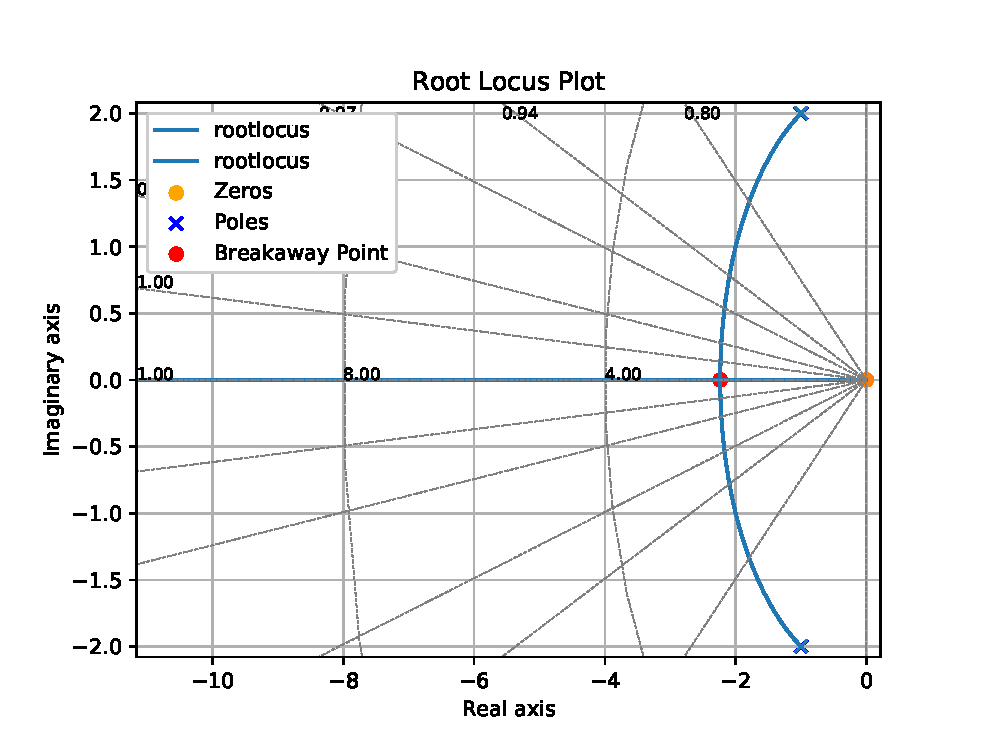
\includegraphics[width=\columnwidth]{./figs/ee18btech11046.eps}

\begin{lstlisting}
codes/ee18btech11046.py
\end{lstlisting}    

\end{enumerate}

